\newcommand{\SimPEG}{\textsc{SimPEG}\xspace}
\renewcommand{\div}{\nabla\cdot}
\newcommand{\grad}{\nabla}
\newcommand{\curl}{{\vec \nabla}\times}
\newcommand {\J}{{\vec J}}
\renewcommand{\H}{{\vec H}}
\newcommand {\E}{{\vec E}}
\newcommand{\siginf}{\sigma_\infty}
\newcommand{\dsig}{\triangle\sigma}
\newcommand{\dcurl}{{\mathbf C}}
\newcommand{\dgrad}{{\mathbf G}}
\newcommand{\Acf}{{\mathbf A_c^f}}
\newcommand{\Ace}{{\mathbf A_c^e}}
\renewcommand{\S}{{\mathbf \Sigma}}
\newcommand{\St}{{\mathbf \Sigma_\tau}}
\newcommand{\T}{{\mathbf T}}
\newcommand{\Tt}{{\mathbf T_\tau}}
\newcommand{\diag}{\mathbf{diag}}
\newcommand{\M}{{\mathbf M}}
\newcommand{\MfMui}{{\M^f_{\mu^{-1}}}}
\newcommand{\MfMuoi}{{\M^f_{\mu_0^{-1}}}}
\newcommand{\dMfMuI}{{d_m (\M^f_{\mu^{-1}})^{-1}}}
\newcommand{\dMfMuoI}{{d_m (\M^f_{\mu_0^{-1}})^{-1}}}
\newcommand{\MeSig}{{\M^e_\sigma}}
\newcommand{\MeSigInf}{{\M^e_{\sigma_\infty}}}
\newcommand{\MeSigInfEtab}{{\M^e_{\sigma_\infty \bar{\eta}}}}
\newcommand{\MeSigInfEtat}{{\M^e_{\sigma_\infty \peta}}}
\newcommand{\MedSig}{{\M^e_{\triangle\sigma}}}
\newcommand{\MeSigO}{{\M^e_{\sigma_0}}}
\newcommand{\Me}{{\M^e}}
\newcommand{\Js}{\mathbf{J}^s}
\newcommand{\Mes}[1]{{\M^e_{#1}}}
\newcommand{\Mee}{{\M^e_e}}
\newcommand{\Mej}{{\M^e_j}}
\newcommand{\BigO}[1]{\mathcal{O}\bigl(#1\bigr)}
\newcommand{\bE}{\mathbf{E}}
\newcommand{\bEp}{\mathbf{E}^p}
\newcommand{\bB}{\mathbf{B}}
\newcommand{\bBp}{\mathbf{B}^p}
\newcommand{\bEs}{\mathbf{E}^s}
\newcommand{\bBs}{\mathbf{B}^s}
\newcommand{\bH}{\mathbf{H}}
\newcommand{\B}{\vec{B}}
\newcommand{\D}{\vec{D}}
\renewcommand{\H}{\vec{H}}
\newcommand{\s}{\vec{s}}
\newcommand{\bfJ}{\bf{J}}
\newcommand{\vecm}{\vec m}
\renewcommand{\Re}{\mathsf{Re}}
\renewcommand{\Im}{\mathsf{Im}}
\renewcommand {\j}  { {\vec j} }
\newcommand {\h}  { {\vec h} }
\renewcommand {\b}  { {\vec b} }
\newcommand {\e}  { {\vec e} }
\renewcommand {\d}  { {\vec d} }
\renewcommand {\u}  { {\vec u} }

\renewcommand {\dj}  { {\mathbf{j} } }
\renewcommand {\dh}  { {\mathbf{h} } }
\newcommand {\db}  { {\mathbf{b} } }
\newcommand {\de}  { {\mathbf{e} } }

\newcommand{\vol}{\mathbf{v}}
\newcommand{\I}{\vec{I}}
\newcommand{\A}{\mathbf{A}}
\newcommand{\bI}{\mathbf{I}}
\newcommand{\bus}{\mathbf{u}^s}
\newcommand{\brhss}{\mathbf{rhs}_s}
\newcommand{\bup}{\mathbf{u}^p}
\newcommand{\brhs}{\mathbf{rhs}}
%%-------------------------------
\newcommand{\bon}{b^{on}(t)}
\newcommand{\bp}{b^{p}}
\newcommand{\dbondt}{\frac{db^{on}(t)}{dt}}
\newcommand{\dfdt}{\frac{df(t)}{dt}}
\newcommand{\dfdtdsiginf}{\frac{\partial\frac{df(t)}{dt}}{\partial\siginf}}
\newcommand{\dfdsiginf}{\frac{\partial f(t)}{\partial\siginf}}
\newcommand{\dbgdsiginf}{\frac{\partial b^{Impulse}(t)}{\partial\siginf}}
\newcommand{\digint}{\frac{2}{\pi}\int_0^{\infty}}
\newcommand{\Gbiot}{\mathbf{G}_{Biot}}
%%-------------------------------
\newcommand{\peta}{\tilde{\eta}}
\newcommand{\eFmax}{\e^{\ F}_{max}}
\newcommand{\eref}{\e^{\ ref}}
\newcommand{\jref}{\j^{\ ref}}
\newcommand{\dip}{d^{IP}}
\newcommand{\sigpert}{\delta\sigma}
\newcommand{\bzip}{b_z^{IP}}
\newcommand{\dbzdtip}{\frac{\partial b_z^{IP}}{\partial t}}
\newcommand{\boldeta}{\boldsymbol{\eta}}
\newcommand{\boldtau}{\boldsymbol{\tau}}
\newcommand{\boldc}{\boldsymbol{c}}
\newcommand{\boldsiginf}{\boldsymbol{\sigma}_{\infty}}
\newcommand{\boldpeta}{\boldsymbol{\peta}}

\section{Discretization}
\label{app: Discretization}
In this section, we discuss important elements about discretizing Maxwell’s equations in the time-domain with the convolution term shown in eq. (\ref{eq:ohmslaw_time}), to simulate IP effects in time-domain EM data. Appendix A.1 illustrates how convolutionary time-domain Maxwell's equations can be discretized.  Appendix A.2 describes how the singularity of SE conductivity function at $t=0$ is handled. Most of key challenges about this discretization are tackled in \cite{marchant2015} (see page 21), and we have extended his work, applied for Cole-Cole conductivity, to SE conductivity.

\subsection{Maxwell's equations}
\label{app: Maxwell's equations}
The stretched exponential (SE) conductivity provided in eq. (\ref{eq: sigma_se_impulse}) in the time-domain can be rewritten as
\begin{equation}
  \sigma_{se}(t) = \siginf \delta (t) + \dsig (t)
  \label{eq:sigma_time}
\end{equation}
where  $\delta(t)$ is a Dirac-Delta function and $\dsig(t)$ is
\begin{equation}
  \dsig (t) = -\siginf \eta_{se}t^{-1}(\frac{t}{\tau_{se}})^{c_{se}}exp\Big(-(\frac{t}{\tau_{se}})^{c_{se}}\Big)
\end{equation}
Considering a time-dependent conductivity, Ohm's Law can be written as
\begin{equation}
  \j = \sigma_{se}(t) \otimes \e =\int_0^t \sigma(t-u) \e (u) du
  \label{eq:ohmslaw}
\end{equation}
and substituting eq. (\ref{eq:sigma_time}) yields
\begin{equation}
  \j = \siginf \e + \int_0^t \dsig(t-u) \e (u) du
  \label{eq:ohmslaw_two}
\end{equation}
Using the Backward Euler method, we discretize Maxwell's equations in eqs. (\ref{eq:faraday}) and (\ref{eq:ampere}) in time:
\begin{equation}
  \curl \e^{\ (n)} = -\frac{\b^{(n)}-\b^{(n-1)}}{\triangle t^{(n)}}
  \label{eq:faraday_time}
\end{equation}
\begin{equation}
  \curl \mu^{-1} \b^{(n)} - \j^{(n)} = \j_s^{(n)} \\
  \label{eq:ampere_time}
\end{equation}
where $\triangle t^{(n)} = t^{(n)}- t^{(n-1)}$.
To discretize the integral in eq. (\ref{eq:ohmslaw_two}), we use the trapezoidal rule:
\begin{equation}
  \int_{t^{(k-1)}}^{t^{(k)}} \dsig(t-u) \e (u) du
  = \frac{\triangle t^{(k)}}{2} \Big(\dsig (t^{(n)} - t^{(k-1)}) \e^{\ (k-1)} + \dsig (t^{(n)} - t^{(k)}) \e^{\ (k)} \Big)
  \label{eq:convolution_trapezoidal}
\end{equation}
Fig. \ref{fig:convolution_concept} shows a conceptual diagram for this discrete convolution procedure.
Hence eq. (\ref{eq:ohmslaw_two}) can be discretized as
\begin{equation}
  \j^{(n)} = \siginf \e^{\ (n)} +
  \sum_{k=1}^{n} \frac{\triangle t^{(k)}}{2} \Big(\dsig (t^{(n)} - t^{(k-1)}) \e^{\ (k-1)} + \dsig (t^{(n)} - t^{(k)}) \e^{\ (k)} \Big)
  \label{eq:ohmslaw_time_original}
\end{equation}
This can be rewritten as
\begin{equation}
  \j^{(n)} = \Big(\siginf + \gamma (\triangle t^{(n)})\Big)\e^{\ (n)} + \j_{pol}^{(n-1)}
  \label{eq:ohmslaw_time}
\end{equation}
where the polarization current, $\j_{pol}^{(n-1)}$ is
\begin{align}
  \j_{pol}^{(n-1)} = \sum_{k=1}^{n-1} \frac{\triangle t^{(k)}}{2} \Big(\dsig (t^{(n)} - t^{(k-1)}) \e^{\ (k-1)} + \dsig (t^{(n)} - t^{(k)}) \e^{\ (k)} \Big) \nonumber \\
  +  \kappa(\triangle t^{(n)}) \e^{\ (n-1)}
\end{align}
For the simplest case when ($c_{se}=1$), then $\dsig(t=0)$  is well defined and  $\gamma (\triangle t^{(n)})$ and $\kappa (\triangle t^{(n)})$ are respectively:
\begin{equation}
  \gamma(\triangle t^{(n)}) = \frac{\triangle t^{(n)}}{2}\dsig (0),
\end{equation}
\begin{equation}
  \kappa(\triangle t^{(n)}) = \frac{\triangle t^{(n)}}{2} \dsig (\triangle t^{(n)})
\end{equation}
However, when $c_{se}\neq1$, $\dsig(t=0)$ is singular and hence it requires special numerical treatment; this is described in Appendix A.2.

For the discretization, we use a staggered mimetic finite volume approach \cite[]{hyman2002}. Here, boldface with uppercase and lowercase indicate matrices and column vectors, respectively. Further details about the discretization can be found in \cite{haber_book} (see page 31).
Discretizing eqs. (\ref{eq:faraday_time}), (\ref{eq:ampere_time}), and (\ref{eq:ohmslaw_time}) yields
\begin{equation}
  \dcurl \de^{\ (n)} = -\frac{\db^{(n)}-\db^{(n-1)}}{\triangle t^{(n)}}
    \label{eq:faraday_discrete}
\end{equation}
\begin{equation}
  \dcurl \MfMui \db^{(n)} - \Me \dj^{(n)} = \mathbf{s}_e^{(n)}, \\
  \label{eq:ampere_discrete}
\end{equation}
\begin{equation}
  \Me\dj^{(n)} = \Mes{A}^{(n)}\de^{\ (n)} + \dj_{pol}^{(n-1)}
  \label{eq:ohmslaw_discrete}
\end{equation}
where
\begin{align}
  \dj_{pol}^{(n-1)} = \sum_{k=1}^{n-1} \frac{\triangle t^{(k)}}{2} \Big(\Mes{\dsig (n, k-1)} \e^{\ (k-1)} + \Mes{\dsig (n, k)} \de^{\ (k)} \Big) \nonumber \\
  +  \Mes{\kappa} \de^{\ (n-1)}
\end{align}
Here, $\mathbf{C}$ is the discrete edge-curl operator; $\mathbf{M}^e$ and $\mathbf{M}^f$ are the edge and face inner-product matrices, respectively. For an inner-product matrix, the subscript indicates corresponding physical property (e.g. $M^{f}_{\mu^{-1}}$: the face inner-product matrix for $\mu^{-1}$).

Rearranging the above equations to solve for $\de$ yields:
\begin{align}
  \Big(\dcurl^T \MfMui \dcurl + \frac{1}{\triangle t^{(n)}} \Mes{A}^{(n)}\Big) \de^{(n)} \nonumber \\
  = - \frac{1}{\triangle t^{(n)}} (\mathbf{s}_e^{(n)}-\mathbf{s}_e^{(n-1)})
    + \frac{1}{\triangle t^{(n)}} \Me \dj^{(n-1)} - \frac{1}{\triangle t^{(n)}} \dj_{pol}^{(n-1)}
    \label{eq: discrete_e_solution}
\end{align}
By solving the above equation at each time step, we obtain $\de$. The measured data for AEM are often $-db/dt$ , which can be computed as
\begin{equation}
    \mathbf{db/dt} = -\dcurl \de
    \label{eq: discrete_dbdt_from_e}
\end{equation}
The measured data at a receiver loop can be expressed as
\begin{equation}
    \mathbf{d} = \mathbf{P} (-\mathbf{db/dt})
    \label{eq: discrete_dbdt_data}
\end{equation}
where $\mathbf{P}$ is an interpolation matrix, which projects $\mathbf{db/dt}$ fields, defined in a 3D domain, to a receiver location, and samples those fields at the measured time channels. For discretization of eqs. (~\ref{eq: discrete_e_solution}) to (~\ref{eq: discrete_dbdt_data}) we use, \SimPEG's mesh toolbox. The developed code is open-source as a \textsc{SimPEG-EMIP} package (\url{https://github.com/sgkang/simpegEMIP})

\begin{figure}[htb]
  \centering
  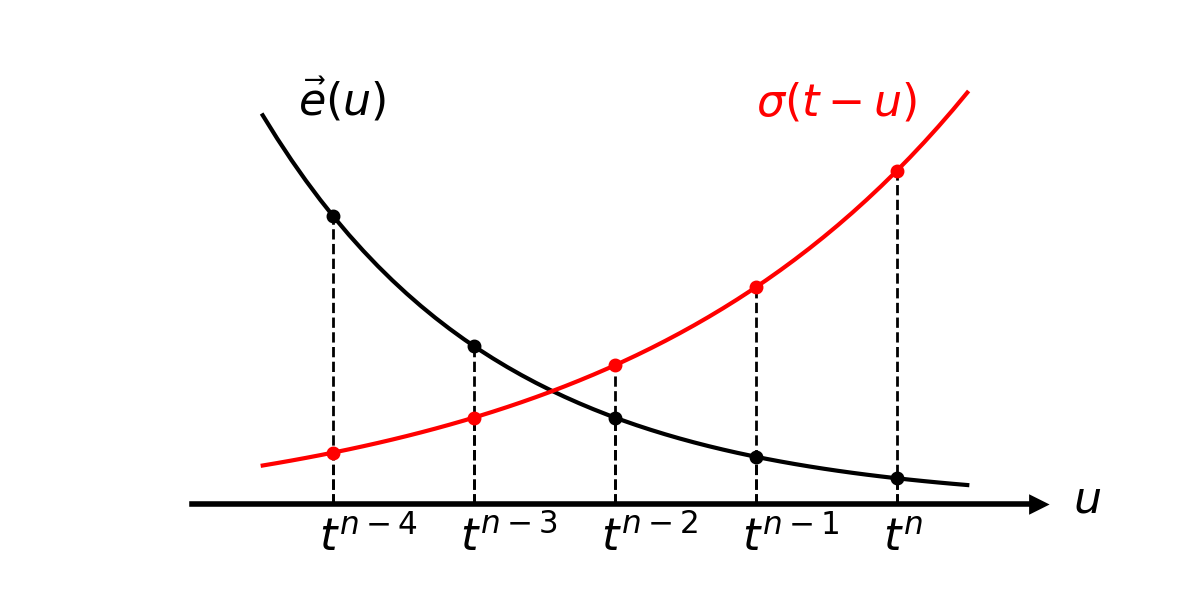
\includegraphics[width=1.0\textwidth]{figures/convolution_concept.png}
  \caption{Conceptual diagram to describe discrete convolution process in eq. (\ref{eq:convolution_trapezoidal})}
  \label{fig:convolution_concept}
\end{figure}

\subsection{Handling the singularity at $\sigma(t=0)$}
\label{app: Handling singularity}
The SE conductivity, $\sigma_{se}(t)$ at $t$=0, is singular, whereas its integral is well-defined, as shown in eq. (\ref{eq: sigma_se_step_off}). When discretizing eq. (\ref{eq:ohmslaw}), this singularity will be problematic. In particular, the issue occurs at the last time segment ($k=n$) of the convolution term in eq. (\ref{eq:ohmslaw_time_original}), which can be written in continuous form:
\begin{equation}
  \int_{t^{n-1}}^{t^{n}} \dsig(u) \e(t-u) du
  \label{eq: convoluation_last_segment}
\end{equation}
This problem also occurs when the Cole-Cole function is used. \cite{marchant2015} (see page 31) tackled this issue by approximating $\e$ at this time segment as a linear function:
\begin{equation}
  \e(t) = \frac{t^{n}-t}{\triangle t^{(n)}} \e^{ \ (n-1)} + \frac{t-t^{n-1}}{\triangle t^{(n)}} \e^{ \ (n-1)}, \ \text{when} \ (t^{(n-1)}\leq t \leq t^{(n)})
\end{equation}
Then by substituting this in to eq. (\ref{eq: convoluation_last_segment}), and evaluating the integration, the discrete form of eq. (\ref{eq: convoluation_last_segment}) is obtained:
\begin{equation}
  \int_{t^{n-1}}^{t^{n}} \dsig(u) \e(t-u) du \simeq
  \kappa(\triangle t^{(n)}) \e^{\ (n-1)} + \gamma(\triangle t^{(n)}) \e^{\ (n)}
\end{equation}

To obtain $\gamma(\triangle t^{(n)})$ and $\kappa(\triangle t^{(n)})$, we use the same trick. Integration of $\dsig(t)$ is not possible, so by Taylor expanding, we obtain an approximate form of $\dsig(t)$ which is valid for small $t$:
\begin{align}
  \dsig (t) = -\siginf \eta_{se}t^{-1}(\frac{t}{\tau_{se}})^{c_{se}}exp\Big(-(\frac{t}{\tau_{se}})^{c_{se}}\Big) \nonumber \\
  \simeq -\siginf \eta_{se}t^{-1}(\frac{t}{\tau_{se}})^{c_{se}}\Big(1-(\frac{t}{\tau_{se}})^{c_{se}}\Big) \nonumber  \\
  = -\siginf \eta_{se}t^{-1}\Big((\frac{t}{\tau_{se}})^{c_{se}}-(\frac{t}{\tau_{se}})^{2c_{se}}\Big)
  \label{eq:se_conductivity_approximate}
\end{align}
By substituting eq. (\ref{eq:se_conductivity_approximate}) into eq. (\ref{eq: convoluation_last_segment}) and evaluating the integral, we finally obtain
\begin{equation}
  \gamma(\triangle t^{(n)}) = \siginf m \Big( \frac{(\triangle t^{(n)})^{c_{se}}}{c_{se}(c_{se}+1)}-
  \frac{(\triangle t^{(n)})^{2c_{se}}}{2c_{se}(2c_{se}+1)\tau_{se}^{c_{se}}} \Big)
\end{equation}
\begin{equation}
  \kappa(\triangle t^{(n)}) = \siginf m \Big( \frac{(\triangle t^{(n)})^{c_{se}}}{c_{se}+1}-
  \frac{(\triangle t^{(n)})^{2c_{se}}}{(2c_{se}+1)\tau_{se}^{c_{se}}} \Big)
\end{equation}

\section{Analytic test}
\label{app: Analytic test}
To test the developed \textsc{SimPEG-EMIP} code, we compare our numerical solution with an analytic solution. A halfspace earth is assumed. The conductivity of the halfspace is 0.05 S/m and its SE parameters are: $\eta_{se}$=0.7, $\tau_{se}$=4ms, $c_{se}$=0.6. Corresponding Cole-Cole parameters are: $\eta_{cc}$=0.8, $\tau_{cc}$=0.005s, $c_{cc}$=0.6.
For the spatial discretization, a 2D cylindrically symmetric mesh is used; the smallest cell size is 6.5m $\times$ 5m.
A horizontal source loop is located 30m above the surface. A step-off waveform is used for the input current and a horizontal receiver loop measuring the voltage (equivalent to -$db_z/dt$) is coincident with the source loop. Data are measured in the off-time over the time-range: 10$^{-2}$-10 ms.
Fig. \ref{fig:analytic_test} shows comparison between analytic and numerical solutions; they match well except for a small shift in the time of the zero-crossing, the two solutions are in good agreement.

\begin{figure}[htb]
  \centering
  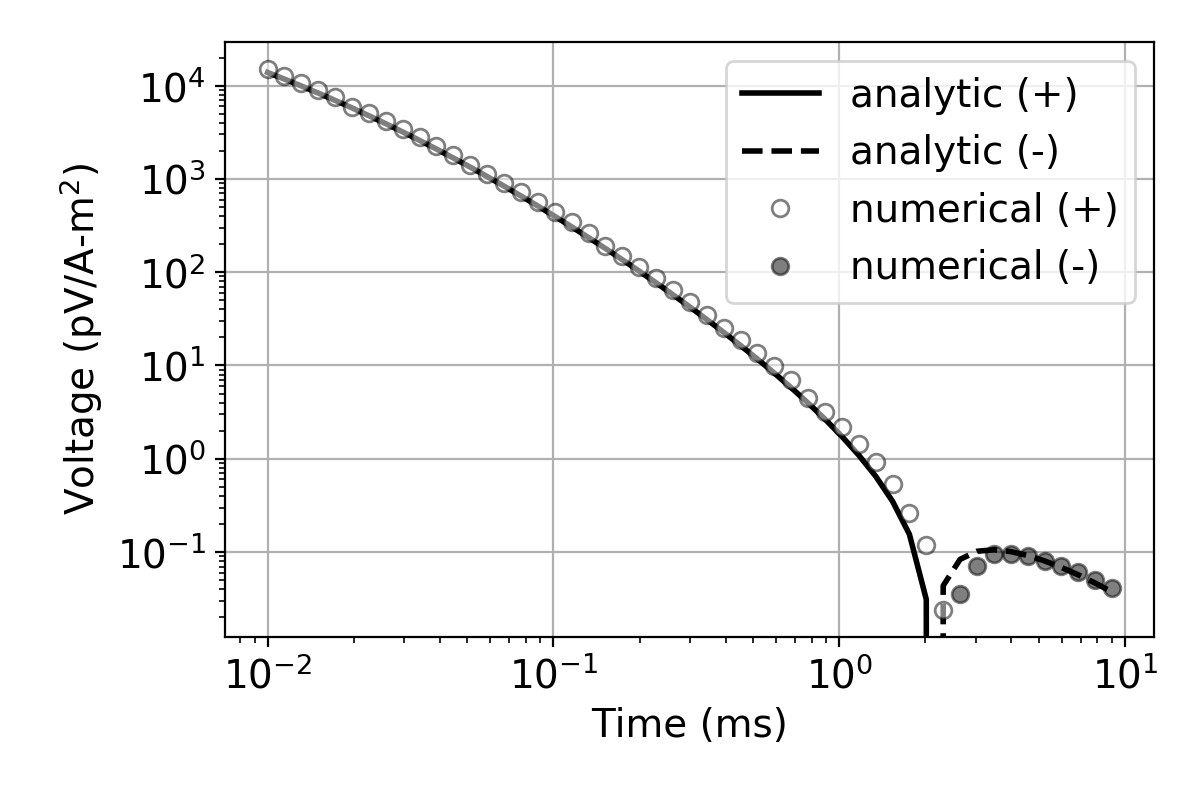
\includegraphics[width=1.0\textwidth]{figures/analytic_test.png}
  \caption{Comparison of numerical and analytic solutions for halfspace earth. SE parameters of the halfspace earth are $\siginf$=0.05S/m, $\eta_{se}$=0.7, $\tau_{se}$=4ms, $c_{se}$=0.6; corresponding Cole-Cole parameters are: $\eta_{cc}$=0.8, $\tau_{cc}$=5ms, $c_{cc}$=0.6. Lines and circles distinguish analytic and numerical solutions.}
  \label{fig:analytic_test}
\end{figure}
